% Auto-generated by experiments/make_toytwin_pgf.py -- clean PGFPlots Boolean-twin figure.
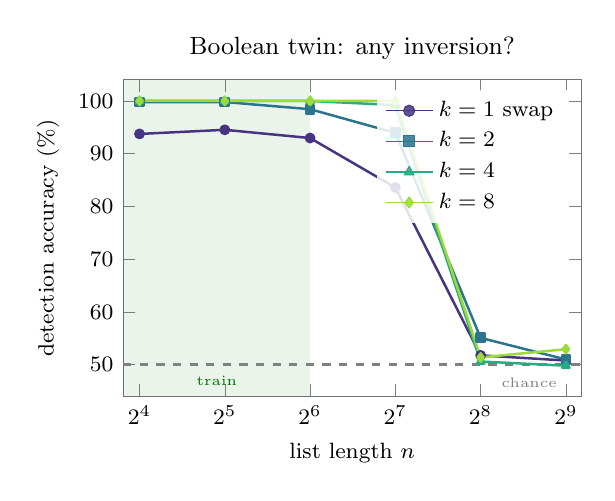
\begin{tikzpicture}
\definecolor{twinA}{RGB}{70,52,128}
\definecolor{twinB}{RGB}{43,116,142}
\definecolor{twinC}{RGB}{37,172,130}
\definecolor{twinD}{RGB}{155,217,60}
\begin{axis}[
  width=7.4cm, height=5.6cm,
  xmode=log, log basis x=2, xmin=14, xmax=580,
  xtick={16,32,64,128,256,512}, xticklabels={$2^4$,$2^5$,$2^6$,$2^7$,$2^8$,$2^9$},
  xlabel={list length $n$}, ylabel={detection accuracy (\%)},
  ymin=44, ymax=104, ytick={50,60,70,80,90,100},
  title={Boolean twin: any inversion?},
  tick label style={font=\footnotesize}, label style={font=\footnotesize},
  title style={font=\small,yshift=-2pt}, axis line style={black!55},
  every axis plot/.append style={line join=round},
  legend cell align=left, legend pos=north east,
  legend style={font=\footnotesize,draw=none,fill opacity=0.85,text opacity=1},
]
\addplot[draw=none,fill=green!45!black,opacity=0.08,forget plot] coordinates {(14,44) (64,44) (64,104) (14,104)} \closedcycle;
\node[font=\tiny,green!45!black] at (axis cs:30,47) {train};
\addplot[gray,dashed,line width=1pt,forget plot] coordinates {(14,50) (580,50)};
\node[font=\tiny,gray] at (axis cs:380,46.5) {chance};
\addplot[twinA,mark=*,mark size=1.5pt,line width=0.9pt,forget plot] coordinates {(16,93.75) (32,94.53) (64,92.97) (128,83.59) (256,51.76) (512,50.78)};
\addplot[twinB,mark=square*,mark size=1.5pt,line width=0.9pt,forget plot] coordinates {(16,99.8) (32,99.8) (64,98.44) (128,93.95) (256,55.08) (512,50.98)};
\addplot[twinC,mark=triangle*,mark size=1.5pt,line width=0.9pt,forget plot] coordinates {(16,100.0) (32,100.0) (64,100.0) (128,99.22) (256,50.59) (512,49.8)};
\addplot[twinD,mark=diamond*,mark size=1.5pt,line width=0.9pt,forget plot] coordinates {(16,100.0) (32,100.0) (64,100.0) (128,100.0) (256,51.37) (512,52.93)};
\addlegendimage{twinA,mark=*}\addlegendentry{$k=1$ swap}
\addlegendimage{twinB,mark=square*}\addlegendentry{$k=2$}
\addlegendimage{twinC,mark=triangle*}\addlegendentry{$k=4$}
\addlegendimage{twinD,mark=diamond*}\addlegendentry{$k=8$}
\end{axis}
\end{tikzpicture}
